\documentclass[11pt]{article}
\title{\textbf{Real data collection}\\
				\large Project for the Internet of Things course @PoliMi Como}
\author{Emanuele Dalla Longa}
\date{2017/11/06}

\usepackage{graphicx}
\usepackage{listings}
\usepackage{amsmath}
\usepackage{hyperref}
\graphicspath{{images/}}
\begin{document}

\maketitle

\section{Introduction}
The aim of this project was to program a TelosB hardware to collect temperature and humidity data from the environment, and broadcast them over the internet, using Node-Red, and analyze them and send the stats via mail. All the code used is available in \href{https://github.com/infinitesnow/IOT2016}{this repository} on GitHub.

\section{Chosen architecture}
I decided to use my Raspberry Pi as a gateway. TelosB was connected over the USB port, and configured to broadcast its output over the serial port. \texttt{node-red} was configured to publish to two online services: Thingspeak (shown in Figure \ref{fig:thingspeak}) and PubNub. From the PubNub channel, I created a Freeboard dashboard to visualize the broadcasted data, as seen in Figure \ref{fig:freeboard}. \texttt{node-red} was configured to send me and a family member a daily report with minimum, maximum and average for each acquired signal for the previous day. All data have been logged into CSV files, which allowed me to plot the data using \texttt{matplotlib}.

\begin{figure}
%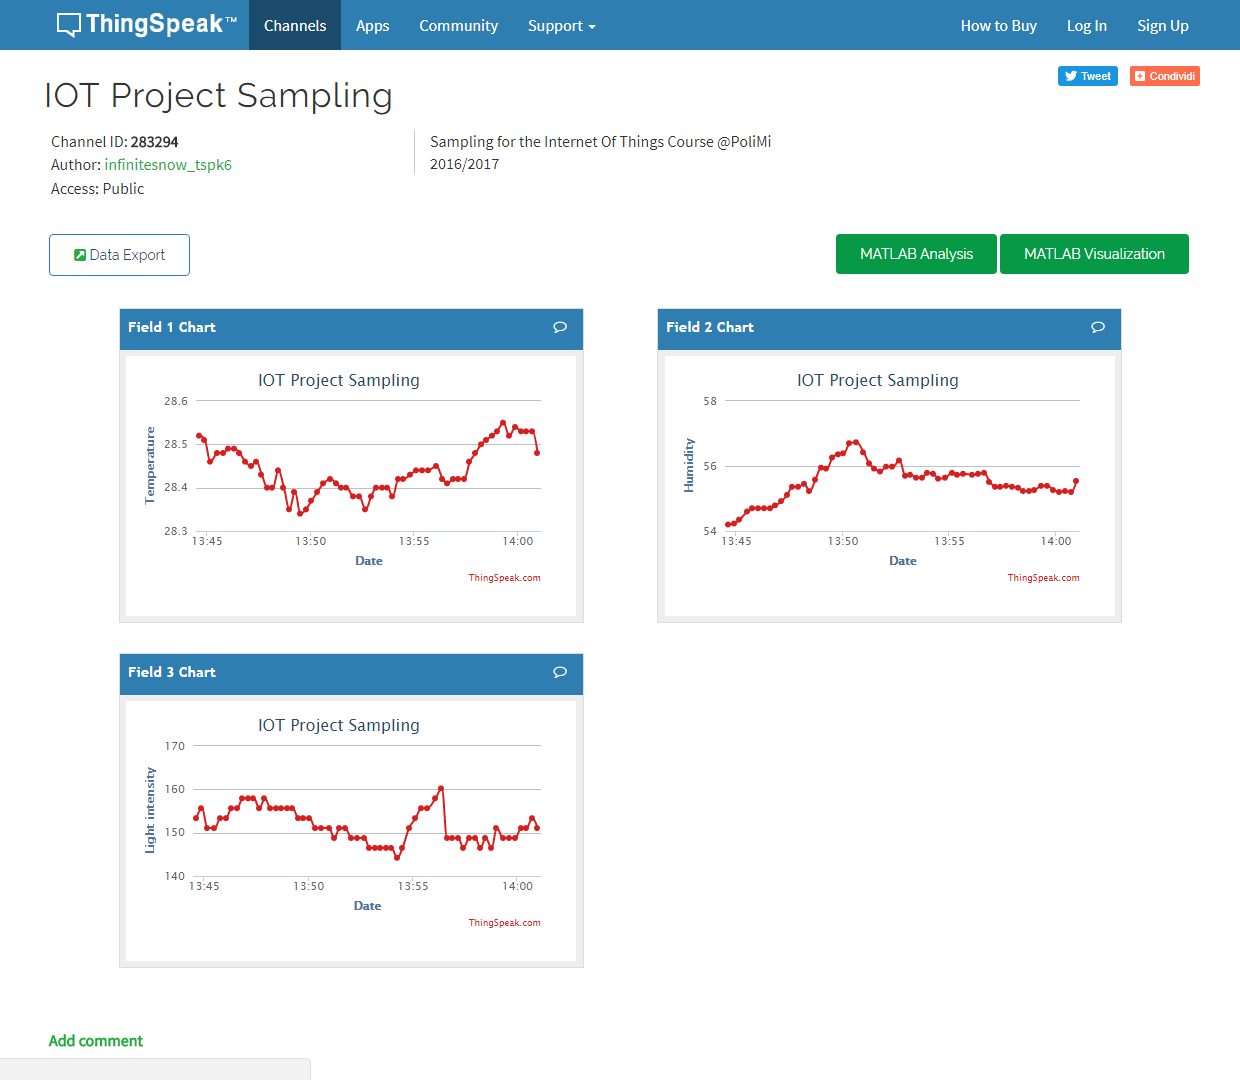
\includegraphics[width=\textwidth]{thingspeak}
\caption{Thingspeak channel}
\label{fig:thingspeak}
\end{figure}

\begin{figure}
%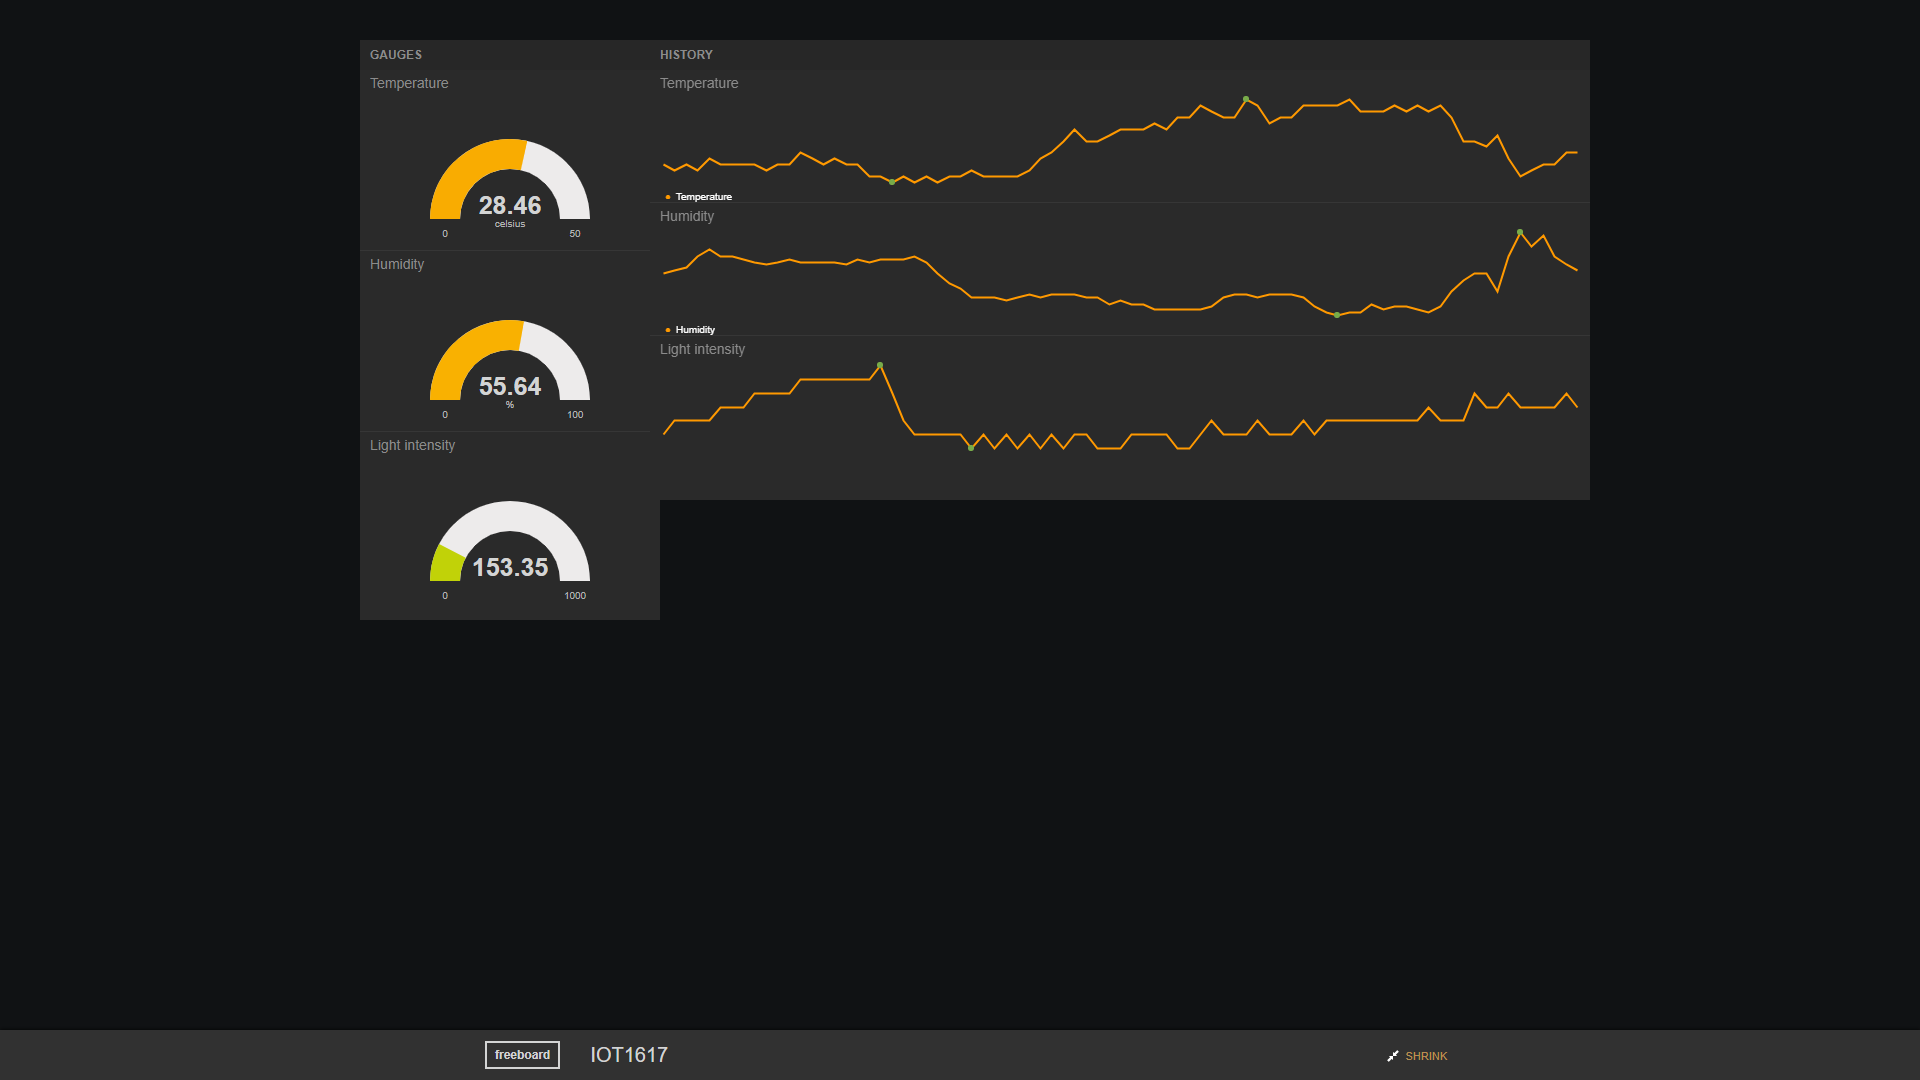
\includegraphics[width=\textwidth]{freeboard}
\caption{Freeboard.io dashboard}
\label{fig:freeboard}
\end{figure}

\section{Reading the serial port}
To read from the serial port, I tried to manually create a script using Python's \texttt{Serial} module, which read chunks of 21 bytes from the input. This worked, but it caused unexpected readings at constant intervals, for reasons which I couldn't understand. Splitting on the \texttt{0x7E} flag byte, which is what the TinyOS library provided in \texttt{tinyos.py} file does, seems to have solved the problem. I switched to \texttt{node-red-node-serialport}, which makes this easy to do and integrates cleanly with \texttt{node-red}.
 
The relevant part of our payload is a \texttt{uint32} counter, and two \texttt{uint16} sensor readings. Here is the relevant part of the parsing done with \texttt{node.js}'s \texttt{Buffer} module, which is output from the \texttt{serial} node

\begin{lstlisting}
var temp = buf.readUInt16BE(13)
var hum = buf.readUInt16BE(15)
\end{lstlisting}

The offsets are such as to strip off the packet header, which is 8 bytes long.

\section{Sensor calibration}
The only sensor I needed to use was a Sensirion SHT11, which provided humidity and temperature readings. I got the transfer function coefficients from the vendor's datasheet. For the humidity, we have:
$$\text{humidity}=c_1+c_2\cdot x +c_3\cdot x^2$$
where
$$c_1= -2.0468$$
$$c_2=  0.0367$$
$$c_3= -1.5955\cdot10^{-6}$$
for the temperature, we have
$$\text{temperature}=d_1+d_2\cdot x$$ 
$$d_1= -40$$
$$d_2=  0.01$$

\section{Sensor data}


\begin{figure}
%\includegraphics[width=\textwidth]{log-2017}
\end{figure}

\end{document}
